\documentclass{standalone}
\usepackage{graphicx}	
\usepackage{amssymb, amsmath}
\usepackage{color}

\usepackage{tikz}
\usetikzlibrary{shapes}
\usepackage{pgfmath}

\definecolor{light}{RGB}{220, 188, 188}
\definecolor{mid}{RGB}{185, 124, 124}
\definecolor{dark}{RGB}{143, 39, 39}
\definecolor{highlight}{RGB}{180, 31, 180}
\definecolor{gray10}{gray}{0.1}
\definecolor{gray20}{gray}{0.2}
\definecolor{gray30}{gray}{0.3}
\definecolor{gray40}{gray}{0.4}
\definecolor{gray60}{gray}{0.6}
\definecolor{gray70}{gray}{0.7}
\definecolor{gray80}{gray}{0.8}
\definecolor{gray90}{gray}{0.9}
\definecolor{gray95}{gray}{0.95}

\newcommand*{\h}{30}

\begin{document}

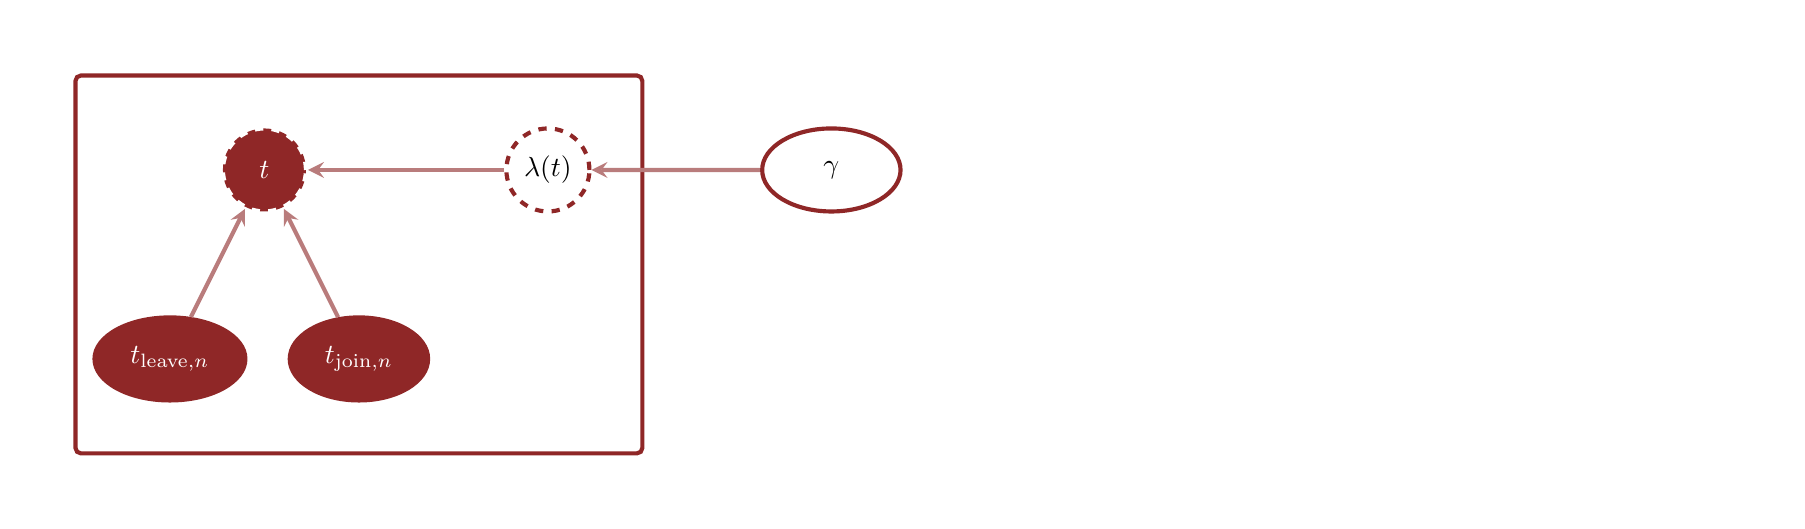
\begin{tikzpicture}[
   scale=0.2,
   obscirc/.style={circle, draw=dark, fill=dark, line width=1.5, text=white,
               inner sep=5, minimum size=\h},
   obsell/.style={ellipse, draw=dark, fill=dark, line width=1.5, text=white,
                  inner sep=5, minimum height=\h, minimum width=50},
   obsrec/.style={rectangle, draw=dark, fill=dark, line width=1.5, text=white,
                  inner sep=5, minimum height=\h, minimum width=\h},
   unobscirc/.style={circle, draw=dark, fill=white, line width=1.5, text=black,
                     inner sep=5, minimum size=\h},
   unobsell/.style={ellipse, draw=dark, fill=white, line width=1.5, text=black,
                    inner sep=5, minimum height=\h}, minimum width=50,
   unobsrec/.style={rectangle, draw=dark, fill=white, line width=1.5, text=black,
                    inner sep=1, minimum height=\h, minimum width=27},
   pushobscirc/.style={circle, draw=white, fill=dark, line width=1.5, dashed, text=white,
                    inner sep=1, minimum size=\h},
   pushunobscirc/.style={circle, draw=dark, fill=white, line width=1.5, dashed, text=black,
                    inner sep=1, minimum size=\h},
   pushell/.style={ellipse, draw=dark, fill=white, line width=1.5, dashed, text=black,
                   inner sep=1, minimum height=\h}
  ]

  % Node Spacing
  \pgfmathsetmacro{\d}{6}
  
  \begin{scope}[shift={(0, 0)}]
    \draw[white] (-8.5 * \d, 0.5 * \d) rectangle (10 * \d, 5.5 * \d);

    %\node (A) at (-3 * \d, 2 * \d) [obsrec] { $x_{n}$ };
    \node (B) at (-3 * \d, 4 * \d) [pushunobscirc] { $\lambda(t)$ };
    
    \node (C) at (-5 * \d, 2 * \d) [obsell] { $t_{\text{join}, n}$ };
    \node (D) at (-7 * \d, 2 * \d) [obsell] { $t_{\text{leave}, n}$ };
    \node (E) at (-6 * \d, 4 * \d) [pushobscirc] { $t$ };
    
    \draw[dark, line width=1.5, rounded corners=2] (-8 * \d, 1 * \d) rectangle (-2 * \d, 5 * \d);

    %\node (F) at (3 * \d, 2 * \d) [obsrec] { $x_{n}$ };
    %\node (G) at (3 * \d, 4 * \d) [pushunobscirc] { $\lambda(t)$ };
    
    %\node (H) at (5 * \d, 2 * \d) [obsell] { $t_{\text{join}, n}$ };
    %\node (J) at (6 * \d, 4 * \d) [pushobscirc] { $t_{\min}$ };
  
    %\draw[dark, line width=1.5, rounded corners=2] (8 * \d, 1 * \d) rectangle (2 * \d, 5 * \d);
    
    %\node (K) at (9 * \d, 4 * \d) [obsrec] { $T_{1}$ };
    
    \node (L) at (0 * \d, 4 * \d) [unobsell] { $\gamma$ };
    
    %\node (M) at (-2 * \d, 7 * \d) [obsrec] { $x_{\text{pred}, n}$ };
    %\node (N) at (0 * \d, 7 * \d) [pushunobscirc] { $\lambda(t)$ };
    %\node (O) at (0 * \d, 9 * \d) [unobscirc] { $t_{\text{pred}}$ };

    %\draw[dark, line width=1.5, rounded corners=2] (-3 * \d, 6 * \d) rectangle (3 * \d, 10 * \d);        
        
    \foreach \B/\E in {L/B,
                       C/E, D/E, B/E} {
      \draw[->, >=stealth, color=mid, line width=1.5] (\B) -- (\E);
    }

  \end{scope}

\end{tikzpicture}

\end{document}  